%\VignetteIndexEntry{faoswsProductionImputation: A package for the imputation of the production domain of the Statistical Working System}
%\VignetteEngine{knitr::knitr}
\documentclass[nojss]{jss}\usepackage[]{graphicx}\usepackage[]{color}
%% maxwidth is the original width if it is less than linewidth
%% otherwise use linewidth (to make sure the graphics do not exceed the margin)
\makeatletter
\def\maxwidth{ %
  \ifdim\Gin@nat@width>\linewidth
    \linewidth
  \else
    \Gin@nat@width
  \fi
}
\makeatother

\definecolor{fgcolor}{rgb}{0.345, 0.345, 0.345}
\newcommand{\hlnum}[1]{\textcolor[rgb]{0.686,0.059,0.569}{#1}}%
\newcommand{\hlstr}[1]{\textcolor[rgb]{0.192,0.494,0.8}{#1}}%
\newcommand{\hlcom}[1]{\textcolor[rgb]{0.678,0.584,0.686}{\textit{#1}}}%
\newcommand{\hlopt}[1]{\textcolor[rgb]{0,0,0}{#1}}%
\newcommand{\hlstd}[1]{\textcolor[rgb]{0.345,0.345,0.345}{#1}}%
\newcommand{\hlkwa}[1]{\textcolor[rgb]{0.161,0.373,0.58}{\textbf{#1}}}%
\newcommand{\hlkwb}[1]{\textcolor[rgb]{0.69,0.353,0.396}{#1}}%
\newcommand{\hlkwc}[1]{\textcolor[rgb]{0.333,0.667,0.333}{#1}}%
\newcommand{\hlkwd}[1]{\textcolor[rgb]{0.737,0.353,0.396}{\textbf{#1}}}%

\usepackage{framed}
\makeatletter
\newenvironment{kframe}{%
 \def\at@end@of@kframe{}%
 \ifinner\ifhmode%
  \def\at@end@of@kframe{\end{minipage}}%
  \begin{minipage}{\columnwidth}%
 \fi\fi%
 \def\FrameCommand##1{\hskip\@totalleftmargin \hskip-\fboxsep
 \colorbox{shadecolor}{##1}\hskip-\fboxsep
     % There is no \\@totalrightmargin, so:
     \hskip-\linewidth \hskip-\@totalleftmargin \hskip\columnwidth}%
 \MakeFramed {\advance\hsize-\width
   \@totalleftmargin\z@ \linewidth\hsize
   \@setminipage}}%
 {\par\unskip\endMakeFramed%
 \at@end@of@kframe}
\makeatother

\definecolor{shadecolor}{rgb}{.97, .97, .97}
\definecolor{messagecolor}{rgb}{0, 0, 0}
\definecolor{warningcolor}{rgb}{1, 0, 1}
\definecolor{errorcolor}{rgb}{1, 0, 0}
\newenvironment{knitrout}{}{} % an empty environment to be redefined in TeX

\usepackage{alltt}
\usepackage{url}
\usepackage[sc]{mathpazo}
\usepackage{geometry}
\geometry{verbose,tmargin=2.5cm,bmargin=2.5cm,lmargin=2.5cm,rmargin=2.5cm}
\setcounter{secnumdepth}{2}
\setcounter{tocdepth}{2}
\usepackage{breakurl}
\usepackage{hyperref}
\usepackage[ruled, vlined]{algorithm2e}
\usepackage{mathtools}
\usepackage{draftwatermark}
\usepackage{float}
\usepackage{placeins}
\usepackage{mathrsfs}
\usepackage{multirow}
%% \usepackage{mathbbm}
\DeclareMathOperator{\sgn}{sgn}
\DeclareMathOperator*{\argmax}{\arg\!\max}



\title{\bf faoswsProductionImputation: A package for the imputation of
  the production domain of the Statistical Working System}

\author{Michael. C. J. Kao\\ Food and Agriculture Organization \\ of
  the United Nations}

\Plainauthor{Michael. C. J. Kao} 

\Plaintitle{faoswsProductionImputation: Package for imputation of the
  production domain of the ESS Statistical Working System}

\Shorttitle{Imputation Module}

\Abstract{ 

  This vignette provides detailed description of the usage of
  functions in the \pkg{faoswsProductionImputation} package. \\
  
  There are three sections to this paper. The opening will describe
  the essential setups required for the package to operate. This is
  then followed by the step-by-step description of each function which
  consist of the whole entire imputation procedure described in the
  methodology paper. Arguements and default setting for each function
  is explained with illustrating example. The final section is for
  technical readers who are interested in building their ensemble
  model, from how to design sensible component model to how to build
  the ensemble.
  
}

\Keywords{Imputation, Linear Mixed Model, Agricultural Production, Ensemble Learning}
\Plainkeywords{Imputation, Linear Mixed Model, Agricultural Production, Ensemble Learning}

\Address{
  Michael. C. J. Kao\\
  Economics and Social Statistics Division (ESS)\\
  Economic and Social Development Department (ES)\\
  Food and Agriculture Organization of the United Nations (FAO)\\
  Viale delle Terme di Caracalla 00153 Rome, Italy\\
  E-mail: \email{michael.kao@fao.org}\\
  URL: \url{https://github.com/mkao006/sws_imputation}
}
\IfFileExists{upquote.sty}{\usepackage{upquote}}{}
\begin{document}




\section{Setup}


Before we begin, we will need to load the required library

\begin{knitrout}
\definecolor{shadecolor}{rgb}{0.969, 0.969, 0.969}\color{fgcolor}\begin{kframe}
\begin{alltt}
\hlcom{## Load libraries}
\hlkwd{library}\hlstd{(faoswsProductionImputation)}
\hlkwd{library}\hlstd{(faoswsExtra)}
\hlkwd{library}\hlstd{(data.table)}
\hlkwd{library}\hlstd{(lattice)}
\end{alltt}
\end{kframe}
\end{knitrout}



To illustrate the functionality of the package, we take the Okra data
set for example. The implementation requires the data to be loaded as
a \textit{data.table} object. This is also the default when data are
queried from the API of the Statistical Working System which we will
refer to as SWS from hereon.

\begin{knitrout}
\definecolor{shadecolor}{rgb}{0.969, 0.969, 0.969}\color{fgcolor}\begin{kframe}
\begin{alltt}
\hlkwd{str}\hlstd{(okrapd)}
\end{alltt}
\begin{verbatim}
## Classes 'data.table' and 'data.frame':	912 obs. of  14 variables:
##  $ areaCode          : int  3 3 3 3 3 3 3 3 3 3 ...
##  $ areaName          : chr  "Albania" "Albania" "Albania" "Albania" ...
##  $ itemCode          : int  430 430 430 430 430 430 430 430 430 430 ...
##  $ itemName          : chr  "Okra" "Okra" "Okra" "Okra" ...
##  $ year              : int  1995 1996 1997 1998 1999 2000 2001 2002 2003 2004 ...
##  $ areaHarvestedValue: num  800 600 750 750 740 780 790 780 700 600 ...
##  $ areaHarvestedFlag : chr  "*" "*" "*" "*" ...
##  $ yieldValue        : num  7.25 8 8 8 7.97 ...
##  $ yieldFlag         : chr  "*" "*" "*" "*" ...
##  $ productionValue   : num  5800 4800 6000 6000 5900 6200 6500 6700 6000 5300 ...
##  $ productionFlag    : chr  "*" "*" "*" "*" ...
##  $ productionFlag2   : logi  NA NA NA NA NA NA ...
##  $ areaHarvestedFlag2: logi  NA NA NA NA NA NA ...
##  $ yieldFlag2        : logi  NA NA NA NA NA NA ...
##  - attr(*, ".internal.selfref")=<externalptr>
\end{verbatim}
\end{kframe}
\end{knitrout}


In addition to the data, the implementation also require a table to
map the hierachical relation of the observation flags. In brief, it
provides a rule for flag aggregation, an example of the table is given
below. For detail treatment and how to create such a table, please see
the vignette of the \pkg{faoswsFlag} package.

\begin{knitrout}
\definecolor{shadecolor}{rgb}{0.969, 0.969, 0.969}\color{fgcolor}\begin{kframe}
\begin{alltt}
\hlstd{swsOldFlagTable} \hlkwb{=} \hlkwd{rbind}\hlstd{(faoswsFlagTable,}
    \hlkwd{data.frame}\hlstd{(}\hlkwc{flagObservationStatus} \hlstd{=} \hlkwd{c}\hlstd{(}\hlstr{"*"}\hlstd{,} \hlstr{"F"}\hlstd{),}
               \hlkwc{flagObservationWeights} \hlstd{=} \hlkwd{c}\hlstd{(}\hlnum{0.9}\hlstd{,} \hlnum{0.6}\hlstd{)))}
\hlstd{swsOldFlagTable[swsOldFlagTable}\hlopt{$}\hlstd{flagObservationStatus} \hlopt{==} \hlstr{"E"}\hlstd{,}
                \hlstr{"flagObservationWeights"}\hlstd{]} \hlkwb{=} \hlnum{0.55}
\hlstd{swsOldFlagTable}
\end{alltt}
\begin{verbatim}
##   flagObservationStatus flagObservationWeights
## 1                                         1.00
## 2                     T                   0.80
## 3                     E                   0.55
## 4                     I                   0.50
## 5                     M                   0.00
## 6                     *                   0.90
## 7                     F                   0.60
\end{verbatim}
\end{kframe}
\end{knitrout}


\section{Functions}
This section provides the step-by-step usage of functions which are
used to perform imputation, the steps illustrated here replicates the
one-step imputation function \code{imputeProductionDomain}.


\subsection{Data processing}

The first step of the imputation is to remove any previous attempt of
imputation. Even for the same methodology and exact setting, prior
imputation will vary as more information are received over time. This
step is highly recommended but optional and depends on the judgement
of the analyst. \\

To remove the prior imputation, one will need to specify the column
name of the value and correspinding flag; further the flag which
represents prior imputation and a flag representing missing
values. The function will convert the previously imputed value to NA
and the flag from previous imputation to a missing flag.

\begin{knitrout}
\definecolor{shadecolor}{rgb}{0.969, 0.969, 0.969}\color{fgcolor}\begin{kframe}
\begin{alltt}
\hlstd{okraProcessed} \hlkwb{=} \hlkwd{copy}\hlstd{(okrapd)}

\hlcom{## Removing prior imputation for production}
\hlkwd{table}\hlstd{(okraProcessed}\hlopt{$}\hlstd{productionFlag)}
\end{alltt}
\begin{verbatim}
## 
##       *   E   F   M   T 
## 487  21  89 150 131  34
\end{verbatim}
\begin{alltt}
\hlkwd{removeImputation}\hlstd{(}\hlkwc{data} \hlstd{= okraProcessed,}
                 \hlkwc{value} \hlstd{=} \hlstr{"productionValue"}\hlstd{,}
                 \hlkwc{flag} \hlstd{=} \hlstr{"productionFlag"}\hlstd{,}
                 \hlkwc{imputedFlag} \hlstd{=} \hlstr{"E"}\hlstd{,}
                 \hlkwc{naFlag} \hlstd{=} \hlstr{"M"}\hlstd{)}
\hlkwd{table}\hlstd{(okraProcessed}\hlopt{$}\hlstd{productionFlag)}
\end{alltt}
\begin{verbatim}
## 
##       *   F   M   T 
## 487  21 150 220  34
\end{verbatim}
\begin{alltt}
\hlcom{## Removing prior imputation for area harvested}
\hlkwd{table}\hlstd{(okraProcessed}\hlopt{$}\hlstd{areaHarvestedFlag)}
\end{alltt}
\begin{verbatim}
## 
##       *   E   F   M   T 
## 430  27 101 188 131  35
\end{verbatim}
\begin{alltt}
\hlkwd{removeImputation}\hlstd{(}\hlkwc{data} \hlstd{= okraProcessed,}
                 \hlkwc{value} \hlstd{=} \hlstr{"areaHarvestedValue"}\hlstd{,}
                 \hlkwc{flag} \hlstd{=} \hlstr{"areaHarvestedFlag"}\hlstd{,}
                 \hlkwc{imputedFlag} \hlstd{=} \hlstr{"E"}\hlstd{,}
                 \hlkwc{naFlag} \hlstd{=} \hlstr{"M"}\hlstd{)}
\hlkwd{table}\hlstd{(okraProcessed}\hlopt{$}\hlstd{areaHarvestedFlag)}
\end{alltt}
\begin{verbatim}
## 
##       *   F   M   T 
## 430  27 188 232  35
\end{verbatim}
\begin{alltt}
\hlcom{## Removing prior imputation for yield}
\hlkwd{table}\hlstd{(okraProcessed}\hlopt{$}\hlstd{yieldFlag)}
\end{alltt}
\begin{verbatim}
## 
##       *   E   F   M   T 
## 410  22 113 200 131  36
\end{verbatim}
\begin{alltt}
\hlkwd{removeImputation}\hlstd{(}\hlkwc{data} \hlstd{= okraProcessed,}
                 \hlkwc{value} \hlstd{=} \hlstr{"yieldValue"}\hlstd{,}
                 \hlkwc{flag} \hlstd{=} \hlstr{"yieldFlag"}\hlstd{,}
                 \hlkwc{imputedFlag} \hlstd{=} \hlstr{"E"}\hlstd{,}
                 \hlkwc{naFlag} \hlstd{=} \hlstr{"M"}\hlstd{)}
\hlkwd{table}\hlstd{(okraProcessed}\hlopt{$}\hlstd{yieldFlag)}
\end{alltt}
\begin{verbatim}
## 
##       *   F   M   T 
## 410  22 200 244  36
\end{verbatim}
\end{kframe}
\end{knitrout}



After removing prior imputation, the next step is to replace zero
values associating with flag "M" to NA. This is due to the fact that
missing values were represented with a value of zero with a flag of
"M".

\begin{knitrout}
\definecolor{shadecolor}{rgb}{0.969, 0.969, 0.969}\color{fgcolor}\begin{kframe}
\begin{alltt}
\hlkwd{remove0M}\hlstd{(}\hlkwc{data} \hlstd{= okraProcessed,}
         \hlkwc{value} \hlstd{=} \hlstr{"productionValue"}\hlstd{,}
         \hlkwc{flag} \hlstd{=} \hlstr{"productionFlag"}\hlstd{,}
         \hlkwc{naFlag} \hlstd{=} \hlstr{"M"}\hlstd{)}

\hlkwd{remove0M}\hlstd{(}\hlkwc{data} \hlstd{= okraProcessed,}
         \hlkwc{value} \hlstd{=} \hlstr{"areaHarvestedValue"}\hlstd{,}
         \hlkwc{flag} \hlstd{=} \hlstr{"areaHarvestedFlag"}\hlstd{,}
         \hlkwc{naFlag} \hlstd{=} \hlstr{"M"}\hlstd{)}

\hlkwd{remove0M}\hlstd{(}\hlkwc{data} \hlstd{= okraProcessed,}
         \hlkwc{value} \hlstd{=} \hlstr{"yieldValue"}\hlstd{,}
         \hlkwc{flag} \hlstd{=} \hlstr{"yieldFlag"}\hlstd{,}
         \hlkwc{naFlag} \hlstd{=} \hlstr{"M"}\hlstd{)}
\end{alltt}
\end{kframe}
\end{knitrout}


In order for the linear mixed model to fit successfully, at least one
observation is required for each country. Thus, this function removes
countries which contains no information or no observation at all.

\begin{knitrout}
\definecolor{shadecolor}{rgb}{0.969, 0.969, 0.969}\color{fgcolor}\begin{kframe}
\begin{alltt}
\hlstd{okraProcessed} \hlkwb{=}
    \hlkwd{removeNoInfo}\hlstd{(}\hlkwc{data} \hlstd{= okraProcessed,}
                 \hlkwc{flag} \hlstd{=} \hlstr{"yieldFlag"}\hlstd{,}
                 \hlkwc{value} \hlstd{=} \hlstr{"yieldValue"}\hlstd{,}
                 \hlkwc{byKey} \hlstd{=} \hlstr{"areaCode"}\hlstd{)}
\end{alltt}
\end{kframe}
\end{knitrout}


The function \code{processProductionDomain} is a wrapper to execute
all the data processing above.

\begin{knitrout}
\definecolor{shadecolor}{rgb}{0.969, 0.969, 0.969}\color{fgcolor}\begin{kframe}
\begin{alltt}
\hlstd{okraProcessed} \hlkwb{=}
    \hlkwd{processProductionDomain}\hlstd{(}\hlkwc{data} \hlstd{= okrapd,}
                           \hlkwc{productionValue} \hlstd{=} \hlstr{"productionValue"}\hlstd{,}
                           \hlkwc{areaHarvestedValue} \hlstd{=}
                               \hlstr{"areaHarvestedValue"}\hlstd{,}
                           \hlkwc{yieldValue} \hlstd{=} \hlstr{"yieldValue"}\hlstd{,}
                           \hlkwc{yearValue} \hlstd{=} \hlstr{"year"}\hlstd{,}
                           \hlkwc{productionObservationFlag} \hlstd{=}
                               \hlstr{"productionFlag"}\hlstd{,}
                           \hlkwc{areaHarvestedObservationFlag} \hlstd{=}
                               \hlstr{"areaHarvestedFlag"}\hlstd{,}
                           \hlkwc{yieldObservationFlag} \hlstd{=} \hlstr{"yieldFlag"}\hlstd{,}
                           \hlkwc{productionMethodFlag} \hlstd{=}
                               \hlstr{"productionFlag2"}\hlstd{,}
                           \hlkwc{areaHarvestedMethodFlag} \hlstd{=}
                               \hlstr{"areaHarvestedFlag2"}\hlstd{,}
                           \hlkwc{yieldMethodFlag} \hlstd{=} \hlstr{"yieldFlag2"}\hlstd{,}
                           \hlkwc{removePriorImputation} \hlstd{=} \hlnum{TRUE}\hlstd{,}
                           \hlkwc{removeConflictValues} \hlstd{=} \hlnum{TRUE}\hlstd{,}
                           \hlkwc{imputedFlag} \hlstd{=} \hlstr{"E"}\hlstd{,}
                           \hlkwc{naFlag} \hlstd{=} \hlstr{"M"}\hlstd{,}
                           \hlkwc{byKey} \hlstd{=} \hlstr{"areaCode"}\hlstd{)}
\end{alltt}
\end{kframe}
\end{knitrout}


\subsection{Imputation}

Now we are ready to perform the imputation. Recalling the methodology
paper, the yield is imputed first. The function \code{imputeYield}
allows the user to specify a desirable formula for the linear mixed
model; otherwise the default linear mixed model with spline will be
used. If the default model is used, the \code{maxdf} sets the maximum
degree of freedom for the B-spline to be tested. The argument
\code{imputationFlag} and \code{newMethodFlag} corresponds to the new
observation status flag and method flag to be assigned for those
values that are imputed.


\begin{knitrout}
\definecolor{shadecolor}{rgb}{0.969, 0.969, 0.969}\color{fgcolor}\begin{kframe}
\begin{alltt}
\hlkwd{imputeYield}\hlstd{(}\hlkwc{yieldValue} \hlstd{=} \hlstr{"yieldValue"}\hlstd{,}
            \hlkwc{yieldObservationFlag} \hlstd{=} \hlstr{"yieldFlag"}\hlstd{,}
            \hlkwc{yieldMethodFlag} \hlstd{=} \hlstr{"yieldFlag2"}\hlstd{,}
            \hlkwc{yearValue} \hlstd{=} \hlstr{"year"}\hlstd{,}
            \hlkwc{imputationFlag} \hlstd{=} \hlstr{"I"}\hlstd{,}
            \hlkwc{newMethodFlag} \hlstd{=} \hlstr{"e"}\hlstd{,}
            \hlkwc{maxdf} \hlstd{=} \hlnum{5}\hlstd{,}
            \hlkwc{byKey} \hlstd{=} \hlstr{"areaCode"}\hlstd{,}
            \hlkwc{data} \hlstd{= okraProcessed)}
\end{alltt}
\end{kframe}
\end{knitrout}


After the imputation of yield, we proceed to impute the production.The
function \code{imputeProduction} function actually compose of two
steps. During the first step, the entries where the imputed yield can
be matched with an existing area harested value are identified, this
in turn, enable us to compute the production. If no value for area
harvested is available, then the function proceed to impute the
remaining production values with ensemble learning. The argument
required is largely similar to those of the \code{imputeYield}
function, however, additional parameters are required for the
implementation of the ensemble model. A list of \textbf{component
  model} is required, and whether the weights of each component model
should be restricted to the specified ceiling for weight
allocation. See the next section for more detail.

\begin{knitrout}
\definecolor{shadecolor}{rgb}{0.969, 0.969, 0.969}\color{fgcolor}\begin{kframe}
\begin{alltt}
\hlkwd{imputeProduction}\hlstd{(}\hlkwc{productionValue} \hlstd{=} \hlstr{"productionValue"}\hlstd{,}
                 \hlkwc{productionObservationFlag} \hlstd{=} \hlstr{"productionFlag"}\hlstd{,}
                 \hlkwc{productionMethodFlag} \hlstd{=} \hlstr{"productionFlag2"}\hlstd{,}
                 \hlkwc{areaHarvestedValue} \hlstd{=} \hlstr{"areaHarvestedValue"}\hlstd{,}
                 \hlkwc{areaHarvestedObservationFlag} \hlstd{=} \hlstr{"areaHarvestedFlag"}\hlstd{,}
                 \hlkwc{yieldValue} \hlstd{=} \hlstr{"yieldValue"}\hlstd{,}
                 \hlkwc{yieldObservationFlag} \hlstd{=} \hlstr{"yieldFlag"}\hlstd{,}
                 \hlkwc{newMethodFlag} \hlstd{=} \hlstr{"e"}\hlstd{,}
                 \hlkwc{data} \hlstd{= okraProcessed,}
                 \hlkwc{restrictWeights} \hlstd{=} \hlnum{TRUE}\hlstd{,}
                 \hlkwc{maximumWeights} \hlstd{=} \hlnum{0.7}\hlstd{,}
                 \hlkwc{byKey} \hlstd{=} \hlstr{"areaCode"}\hlstd{,}
                 \hlkwc{flagTable} \hlstd{= swsOldFlagTable)}
\end{alltt}
\end{kframe}
\end{knitrout}


Finally, we can balance the area harvested after both production and
yield have been imputed.

\begin{knitrout}
\definecolor{shadecolor}{rgb}{0.969, 0.969, 0.969}\color{fgcolor}\begin{kframe}
\begin{alltt}
\hlkwd{balanceAreaHarvested}\hlstd{(}\hlkwc{productionValue} \hlstd{=} \hlstr{"productionValue"}\hlstd{,}
                     \hlkwc{productionObservationFlag} \hlstd{=} \hlstr{"productionFlag"}\hlstd{,}
                     \hlkwc{areaHarvestedValue} \hlstd{=} \hlstr{"areaHarvestedValue"}\hlstd{,}
                     \hlkwc{areaHarvestedObservationFlag} \hlstd{=} \hlstr{"areaHarvestedFlag"}\hlstd{,}
                     \hlkwc{areaHarvestedMethodFlag} \hlstd{=} \hlstr{"areaHarvestedFlag2"}\hlstd{,}
                     \hlkwc{yieldValue} \hlstd{=} \hlstr{"yieldValue"}\hlstd{,}
                     \hlkwc{yieldObservationFlag} \hlstd{=} \hlstr{"yieldFlag"}\hlstd{,}
                     \hlkwc{newMethodFlag} \hlstd{=} \hlstr{"e"}\hlstd{,}
                     \hlkwc{data} \hlstd{= okraProcessed,}
                     \hlkwc{flagTable} \hlstd{= swsOldFlagTable)}
\end{alltt}
\end{kframe}
\end{knitrout}


The full procedure outlined in this section can be performed by a
single function \code{imputeProductionDomain}.


\begin{knitrout}
\definecolor{shadecolor}{rgb}{0.969, 0.969, 0.969}\color{fgcolor}\begin{kframe}
\begin{alltt}
\hlkwd{system.time}\hlstd{(}
    \hlstd{\{}
        \hlstd{imputedokrapd} \hlkwb{=}
            \hlkwd{imputeProductionDomain}\hlstd{(}\hlkwc{data} \hlstd{= okrapd,}
                                   \hlkwc{productionValue} \hlstd{=} \hlstr{"productionValue"}\hlstd{,}
                                   \hlkwc{areaHarvestedValue} \hlstd{=}
                                       \hlstr{"areaHarvestedValue"}\hlstd{,}
                                   \hlkwc{yieldValue} \hlstd{=} \hlstr{"yieldValue"}\hlstd{,}
                                   \hlkwc{yearValue} \hlstd{=} \hlstr{"year"}\hlstd{,}
                                   \hlkwc{productionObservationFlag} \hlstd{=}
                                       \hlstr{"productionFlag"}\hlstd{,}
                                   \hlkwc{areaHarvestedObservationFlag} \hlstd{=}
                                       \hlstr{"areaHarvestedFlag"}\hlstd{,}
                                   \hlkwc{yieldObservationFlag} \hlstd{=} \hlstr{"yieldFlag"}\hlstd{,}
                                   \hlkwc{productionMethodFlag} \hlstd{=}
                                       \hlstr{"productionFlag2"}\hlstd{,}
                                   \hlkwc{areaHarvestedMethodFlag} \hlstd{=}
                                       \hlstr{"areaHarvestedFlag2"}\hlstd{,}
                                   \hlkwc{yieldMethodFlag} \hlstd{=} \hlstr{"yieldFlag2"}\hlstd{,}
                                   \hlkwc{flagTable} \hlstd{= swsOldFlagTable,}
                                   \hlkwc{removePriorImputation} \hlstd{=} \hlnum{TRUE}\hlstd{,}
                                   \hlkwc{removeConflictValues} \hlstd{=} \hlnum{TRUE}\hlstd{,}
                                   \hlkwc{imputedFlag} \hlstd{=} \hlstr{"E"}\hlstd{,}
                                   \hlkwc{imputationFlag} \hlstd{=} \hlstr{"I"}\hlstd{,}
                                   \hlkwc{newMethodFlag} \hlstd{=} \hlstr{"e"}\hlstd{,}
                                   \hlkwc{naFlag} \hlstd{=} \hlstr{"M"}\hlstd{,}
                                   \hlkwc{maxdf} \hlstd{=} \hlnum{5}\hlstd{,}
                                   \hlkwc{byKey} \hlstd{=} \hlstr{"areaCode"}\hlstd{,}
                                   \hlkwc{restrictWeights} \hlstd{=} \hlnum{TRUE}\hlstd{,}
                                   \hlkwc{maximumWeights} \hlstd{=} \hlnum{0.7}\hlstd{)}
    \hlstd{\}}
    \hlstd{)}
\end{alltt}
\begin{verbatim}
## Initializing ... 
## Imputing Yield ...
## Model with 2 degree of freedom is selected
## Number of values imputed:  195 
## Number of values still missing:  0 
## Imputing Production ...
## Number of values imputed:  171 
## Number of values still missing:  0 
## Imputing Area Harvested ...
## Number of values imputed:  194 
## Number of values still missing:  0
##    user  system elapsed 
##   86.54   91.21   78.62
\end{verbatim}
\end{kframe}
\end{knitrout}




\section{Ensemble model}
Here we provide some details of how to implement user specific
ensemble models.\\

First of all, the component model need to take a vector of values and
return the fitted values. If the model failed or if the fit does not
correspond to values in the codomain, then return a vector of NA equal
to the length of the input.\\

Shown below is the default logitstic model in the package, the model
will return a vector of NA if there are no observations at both
tail. It is the analyst's job to ensure the component models return
sensible values. For example, negative values are nonsensical for
production, and in the current implementation negative values are
replaced with zero.

\begin{knitrout}
\definecolor{shadecolor}{rgb}{0.969, 0.969, 0.969}\color{fgcolor}\begin{kframe}
\begin{alltt}
\hlstd{defaultLogistic} \hlkwb{=} \hlkwa{function} \hlstd{(}\hlkwc{x}\hlstd{)\{}
    \hlstd{time} \hlkwb{=} \hlnum{1}\hlopt{:}\hlkwd{length}\hlstd{(x)}
    \hlstd{xmax} \hlkwb{=} \hlkwd{max}\hlstd{(x,} \hlkwc{na.rm} \hlstd{=} \hlnum{TRUE}\hlstd{)}
    \hlstd{x.scaled} \hlkwb{=} \hlstd{x}\hlopt{/}\hlstd{xmax}
    \hlstd{logisticModel} \hlkwb{=} \hlkwd{glm}\hlstd{(}\hlkwc{formula} \hlstd{= x.scaled} \hlopt{~} \hlstd{time,} \hlkwc{family} \hlstd{=} \hlstr{"binomial"}\hlstd{)}
    \hlstd{logisticFit} \hlkwb{=} \hlkwd{predict}\hlstd{(logisticModel,}
                          \hlkwc{newdata} \hlstd{=} \hlkwd{data.frame}\hlstd{(}\hlkwc{time} \hlstd{= time),}
                          \hlkwc{type} \hlstd{=} \hlstr{"response"}\hlstd{)} \hlopt{*} \hlstd{xmax}
    \hlstd{midpoint} \hlkwb{=} \hlopt{-}\hlkwd{coef}\hlstd{(logisticModel)[}\hlnum{1}\hlstd{]}\hlopt{/}\hlkwd{coef}\hlstd{(logisticModel)[}\hlnum{2}\hlstd{]}
    \hlkwa{if} \hlstd{(}\hlkwd{length}\hlstd{(}\hlkwd{na.omit}\hlstd{(x[time} \hlopt{<} \hlstd{midpoint]))} \hlopt{<} \hlnum{1} \hlopt{|}
        \hlkwd{length}\hlstd{(}\hlkwd{na.omit}\hlstd{(x[time} \hlopt{>} \hlstd{midpoint]))} \hlopt{<} \hlnum{1}\hlstd{)}
        \hlstd{logisticFit} \hlkwb{=} \hlkwd{rep}\hlstd{(}\hlnum{NA}\hlstd{,} \hlkwd{length}\hlstd{(x))}
    \hlstd{logisticFit}
\hlstd{\}}
\end{alltt}
\end{kframe}
\end{knitrout}

After defining the component models, the next step is to combine the
models into a list. The support functions in the package will then
take care of the rest.

\begin{knitrout}
\definecolor{shadecolor}{rgb}{0.969, 0.969, 0.969}\color{fgcolor}\begin{kframe}
\begin{alltt}
\hlstd{myModel} \hlkwb{=} \hlkwd{list}\hlstd{(defaultMean, defaultLm, defaultExp,}
        \hlstd{defaultLogistic, defaultLoess, defaultSpline, defaultArima,}
        \hlstd{defaultMars, defaultNaive)}
\end{alltt}
\end{kframe}
\end{knitrout}

Here we take the Okra production value of Bahrain as an
illustration. After the component models has been designed and
inserted into a list, we can first compute the fits and weights then
combine it to form the ensemble with the following functions.

\begin{knitrout}
\definecolor{shadecolor}{rgb}{0.969, 0.969, 0.969}\color{fgcolor}\begin{kframe}
\begin{alltt}
\hlstd{bahrainExample} \hlkwb{=} \hlstd{okraProcessed[areaName} \hlopt{==} \hlstr{"Bahrain"}\hlstd{, productionValue]}

\hlcom{## Compute fit for all component models}
\hlstd{modelFits} \hlkwb{=}
    \hlkwd{computeEnsembleFit}\hlstd{(}\hlkwc{x} \hlstd{= bahrainExample,} \hlkwc{ensembleModel} \hlstd{= myModel)}

\hlcom{## Calculate the weight for each component model}
\hlstd{modelWeights} \hlkwb{=}
    \hlkwd{computeEnsembleWeight}\hlstd{(}\hlkwc{x} \hlstd{= bahrainExample,}
                          \hlkwc{fits} \hlstd{= modelFits,}
                          \hlkwc{restrictWeights} \hlstd{=} \hlnum{TRUE}\hlstd{,}
                          \hlkwc{maximumWeights} \hlstd{=} \hlnum{0.7}\hlstd{)}

\hlcom{## Combine the models to obtain the ensemble}
\hlstd{ensembleFit} \hlkwb{=} \hlkwd{computeEnsemble}\hlstd{(modelFits, modelWeights)}
\end{alltt}
\end{kframe}
\end{knitrout}

A one-step wrapper function is also available.  An optional arguement
for ensemble weight is available. You can specify whether to restrict
the weights of a single model. In this example, the default restricts
the weight and set the maximum weight of a model can take to 0.7.

\begin{knitrout}
\definecolor{shadecolor}{rgb}{0.969, 0.969, 0.969}\color{fgcolor}\begin{kframe}
\begin{alltt}
\hlstd{fijiExample} \hlkwb{=} \hlstd{okraProcessed[areaName} \hlopt{==} \hlstr{"Fiji Islands"}\hlstd{, productionValue]}
\hlstd{ensembleFit} \hlkwb{=}
    \hlkwd{ensembleImpute}\hlstd{(}\hlkwc{x} \hlstd{= fijiExample,}
                   \hlkwc{restrictWeights} \hlstd{=} \hlnum{TRUE}\hlstd{,}
                   \hlkwc{maximumWeights} \hlstd{=} \hlnum{0.7}\hlstd{,}
                   \hlkwc{plot} \hlstd{=} \hlnum{TRUE}\hlstd{)}
\end{alltt}
\end{kframe}

{\centering 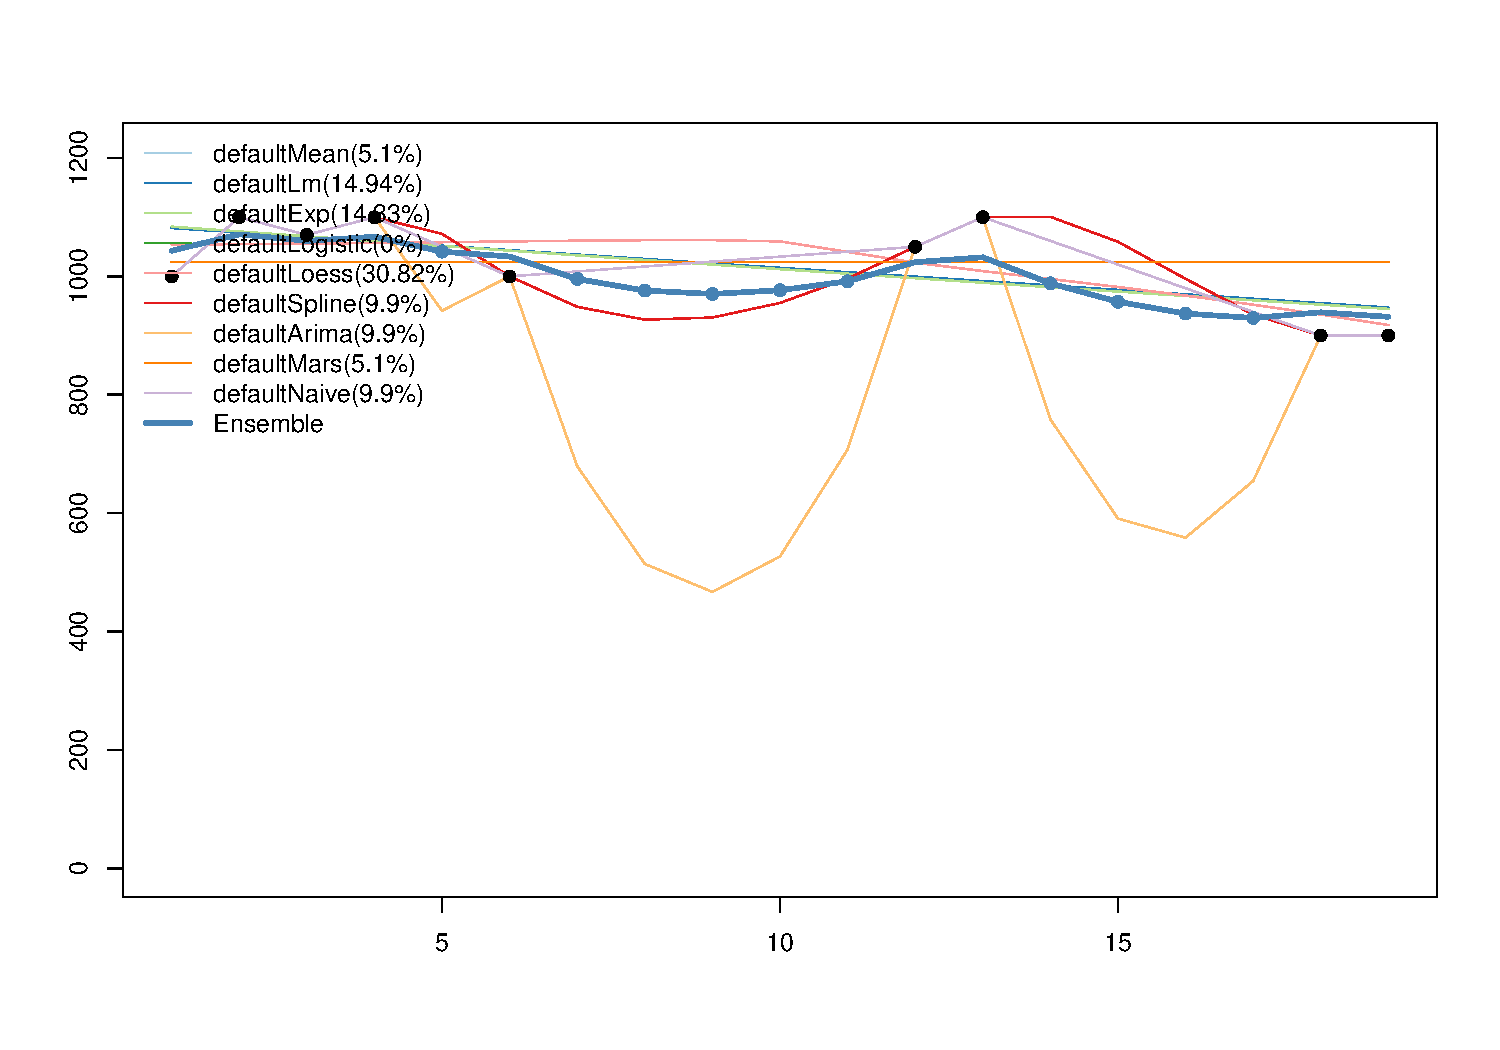
\includegraphics[width=\maxwidth]{figure/ensemble-imputation} 

}



\end{knitrout}


\end{document}
